\chapter{Marco Te\'orico}

\subsection{Computaci\'on Ubicua}

En 1991 Mark Weiser investigador en la Computer Science Laboratory en Xerox PARC publicaba un articulo llamado "La computadora para el siglo 21".

Para Weiser existen 3 etapas de la computación:

\begin{itemize}
    \item La era de los Mainframes o estaciones de trabajo.
    \item La era del computador personal.
    \item La era del computo ubicuo.
\end{itemize}

El computo ubicuo según Weiser, constituye la tercera ola de la computación. Básicamente es un entorno tecnológico en donde dispositivos de diferentes tamaños y funcionalidades, pueden conectarse y usarse en conjunto para manejar información, de forma que el hombre opera con mayor facilidad sus actividades del mundo cotidiano. Es decir, usar la tecnología a un nivel tan profundo que se desvanece en el tejido de la vida cotidiana, hasta que sea indistinguible.

Por lo tanto, estamos tratando de concebir una nueva forma de pensar acerca de las computadoras en el mundo, una que tenga en cuenta el entorno humano natural y permita que las mismas computadoras se desvanezcan en el fondo del ecosistema. Tal mezcla es una consecuencia fundamental no de la tecnología, sino de la psicología humana. Cuando las personas aprenden algo lo suficientemente bien, dejan de ser conscientes de ello.

La máquina multimedia de hoy, demanda la atención de la pantalla del ordenador, convirtiéndola en un foco de atención en lugar de permitir que se desvanezca en el fondo.

El sentido opuesto del computo ubicuo sería "realidad virtual" debido a que la realidad virtual se centra en un enorme aparato para simular el mundo, en lugar de mejorar de manera invisible el mundo, que ya existe.

Para explicar mejor el concepto de: "se desvance en el medio", podemos utiliza el ejemplo de "motores eléctricos dentro de un carro", están ahí al limpiar el parabrisas, al bloquear o desbloquear las puertas, pero no nos preocupamos de dónde están, sino que interactuamos de manera natural para realizar todas estas acciones. De esta manera el computo ubicuo busca que las computadoras sean invisibles.

Cientos de computadoras en una habitación suena intimidante, pero vendrán a ser invisibles a la conciencia común. La gente simplemente los usará inconscientemente para realizar tareas cotidianas.
El verdadero poder del concepto emerge de la interacción entre todos los dispositivos.

Hay más información disponible a nuestro alcance durante un paseo por el bosque que en cualquier sistema informático, sin embargo, la gente encuentra Un paseo entre árboles relajante y computadoras frustrantes. Máquinas que se adaptan al entorno humano, en lugar de obligar a los humanos a entrar en los suyos, hará que usar una computadora sea tan refrescante como pasear por el bosque.\cite{weiser}

\subsection{Movilidad inform\'atica}

Gracias a lo anterior podemos deducir que nos encontramos en la segunda era de la computación. La era del computador personal que a diferencia con la primera se caracteriza por la "movilidad física".

El usuario del entorno de computación móvil podrá acceder a datos, información u otros objetos lógicos desde cualquier dispositivo en cualquier red mientras esté en movimiento.\cite{asoke}

cliente servidor

Por lo tanto la "movilidad informatica" incluye cualquier dispositivo de computo fácilmente transportable y donde el usuario pueda realizar una tarea en movimiento o desde cualquier lugar en donde se encuentre. 

Usando un dispositivo de computación en una red pública (la web), o corporativa (información comercial) y espacios de información personal (registro médico, libreta de direcciones), etc. Lo que llamaremos aplicativos o aplicaciones.

Para llevarlo al siguiente nivel, el computo ubiquo, es necesario que el portador de la comunicación se extienda a través de medios inalámbricos y por cable. Es decir el dispositivo ubiquo compartira su información con el medio que lo rodea. Existirá tal cantidad de información que será necesario tratarla para sacar estadisticas o parametros que nos fáciliten la vida, incluso para que el dispositivo ubiquo pueda aprender de su propia información recolectada.

\subsection{Smarthphone}

\begin{figure}[bp!]
	\centering
	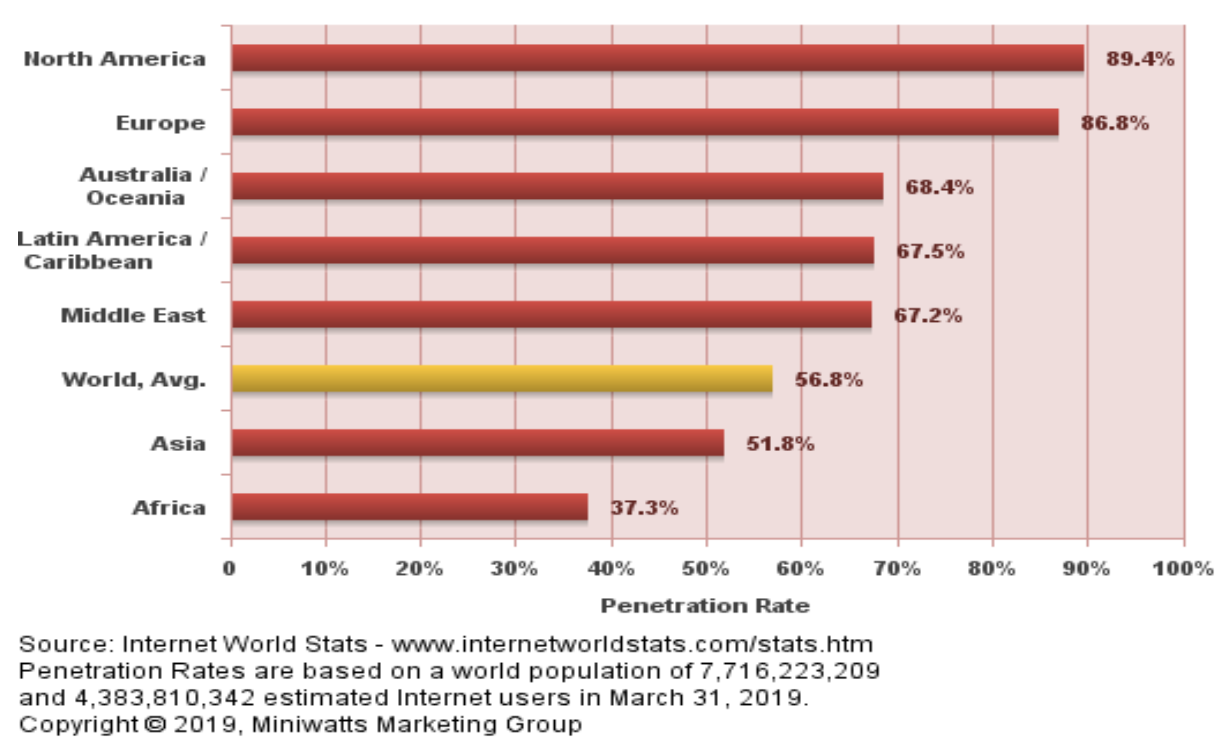
\includegraphics[width=5in]{imgs/internetPenetration19}
	  \caption{Internet World penetration rates by Geographic Regions - March, 2019}
\end{figure}

Actualmente la difusión de la tecnología móvil se ha visto ampliamente extendida principalmente a la penetración de internet en la sociedad \cite{internetPenetration}, así como la disminución en el costo de adquisición de los telefonos inteligentes o smarthphones. Sumado al acceso a la web a través de éstos. Ha detonado sin duda el uso habitual de telefonos inteligentes en nuestra sociedad actual.

Las ventajas de un telefono inteligente van más allá de poder acceder a internet y compartir información mieentras nos desplazamos. Cabe especificar que los telefonos inteligentes cuentan con diversos sensores integrados, como lo son: acelerómetros, giroscopio, sensor de huella, sensor dactilar, bluethoot, magnetómetro, receptor GPS, etc. Mismos que convirten al telefono inteligente en una navaja suiza y nos da un ecosistema fertil para un desarrollar infinidad de aplicativos. Tantos como nuestra imaginación.


\subsection{GPS}

Uno de los sensores principales con los que actualmente cuentan los telefonos intligentes es el receptor GPS. El Gps permite determinar la posición las 24 horas del día, en cualquier lugar del globo, bajo cualquier condición climatológica.\cite{latham}

A través del GPS podemos obtener: latitud, longitud, altitud del dispositivo. A su vez, a partir de estos datos podemos obtener información diversa, como: la velocidad de desplazamiento, la hora exacta, la distancia del dispositivo a un punto dado, si el dispositivo ha entrado a un area específica, si ha salido de un área en específica, principalmente.

\subsubsection{Arquitectura}

El sistema completo se compone de 3 elementos distintos denominados segmentos, los cuales son:

\begin{enumerate}
\item Segmento espacial: lo componen los satélites.
\item Segmento de control: lo componen las estaciones de control.
\item Segmento del usuario: lo componenlos receptores GPS.
\end{enumerate}
\newpage

\paragraph{Segmento espacial.}
 
	Está formado por una constelación de 24 satélites llamados SV (Space Vehicle). Circundan la tierra a 20.2000 km de altitud y forman 6 órbitas diferentes con 4 satélites cada una.
	Cada 24 horas (menos 4 minutos a causa del desplazamiento de la tierra al rededor del sol), se presenta exactamente en el mismo lugar y con la misma configuración respecto a los demás satélites.
	
	\begin{figure}[bp!]
	\centering
	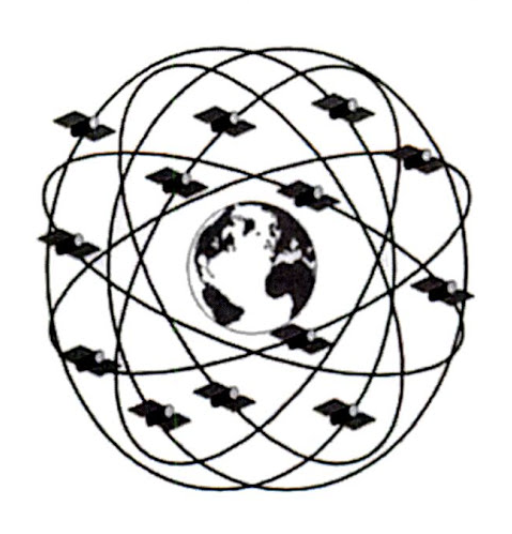
\includegraphics[width=3in]{imgs/24satelites}
	  \caption{La tecnología GPS se basa en un grupo de 24 satélites que emiten señales a la Tierra.}
\end{figure}

	Cada satelite envia un mensaje de navegación indicando su posición orbital así como la hora exacta de la emisión de dicho mensaje.
	
\paragraph{Segmento de control.}

	Se conforma por 5 estaciones de vigilacia y monitorización del sistema GPS, distribuidas al rededor del planeta, incluyendo una estación principal que asegura el correcto funcionamiento del sistema calculando las correcciones a aplicar.
	
	Las cinco estaciones se encuentran en las islas: Hawaii, Kwajalein (islas Marshall), Ascensión, Diego Garcia, en Colorado Springs. Su misión es captar todas las seáles emitidas por los satélites, acumular los mensajes recibidos y transmitir todas las informaciones recogidas a la estación principal.
	
\begin{figure}[bp!]
	\centering
	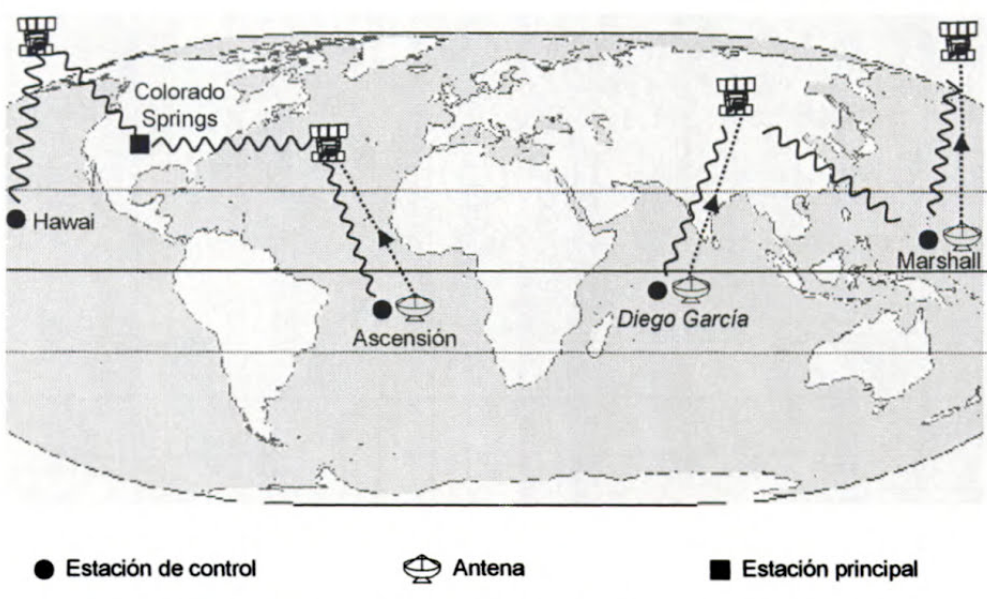
\includegraphics[width=5in]{imgs/estacionControl}
	  \caption{Estaciones de control.}
\end{figure}
	
\paragraph{Segmento del usuario.}

	Comprende la antena de recepción y el receptor (microprocesador) GPS. Podemos obtener información sobre posición, velocidad, ruta, hora y fecha.

\subsubsection{Servicio}

Existen dos tipos de servicio que brinda el sistema de posicionamiento global, uno público SPS (servicio de posicionamiento estándar) destinado a usuarios civiles en una sola frecuencia. El otro tipo de servicio es privado el PPS (servicio de posicionamiento preciso) este, está reservado para uso exclusivo del ejercito de USA.

El primero (SPS) está degradado con propósito de proteger la seguridad USA, la degradación consiste en una pequeña modificación del valor del reloj del satélite con ayuda de un generador pseudoaleatorio. Con un error inferior a 100 mts en horizontal y 156 mts en vertical, así como la hora con una precisión de 340 nanosegundos. El ejercito de USA puede modificar la degradación en caso de amenaza o un posible caso de guerra.

Por otro lado el PPS cuenta con un error inferior a los 21 mtrs en horizontal, de 27.7 mtrs en vertical y la hora con una precisión de 100 nanosegundos.


